\section{Irregular Sensor Data Compression}
{{\footnotesize
\begin{description}[labelwidth=5em, labelsep=1em, leftmargin=*, align=left, itemsep=0.3em, parsep=0em]
  \item[date:] 2024-05-01
  \item[version:] TODO
  \item[last\_updated:] 2024-05
  \item[expired:] unknown
  \item[valid:] yes
  \item[valid\_date:] TODO
  \item[url:] \href{https://github.com/fastmachinelearning/fastml-science/tree/main/sensor-data-compression}{https://github.com/fastmachinelearning/fastml-science/tree/main/sensor-data-compression}
  \item[doi:] TODO
  \item[domain:] Particle Physics
  \item[focus:] Real-time compression of sparse sensor data with autoencoders
  \item[keywords:]
    - compression
    - autoencoder
    - sparse data
    - irregular sampling
  \item[summary:] This benchmark addresses lossy compression of irregularly sampled
sensor data from particle detectors using real-time autoencoder architectures,
targeting latency-critical applications in physics experiments.

  \item[licensing:] TODO
  \item[task\_types:]
    - Compression
  \item[ai\_capability\_measured:]
    - Reconstruction quality
    - compression efficiency
  \item[metrics:]
    - MSE
    - Compression ratio
  \item[models:]
    - Autoencoder
    - Quantized autoencoder
  \item[ml\_motif:]
    - Real-time, Image/CV
  \item[type:] Benchmark
  \item[ml\_task:]
    - Unsupervised Learning
  \item[solutions:] TODO
  \item[notes:] Based on synthetic but realistic physics sensor data

  \item[contact.name:] Ben Hawks, Nhan Tran
  \item[contact.email:] unknown
  \item[datasets.links.name:] Custom synthetic irregular sensor dataset
  \item[datasets.links.url:] \href{https://github.com/fastmachinelearning/fastml-science/tree/main/sensor-data-compression}{https://github.com/fastmachinelearning/fastml-science/tree/main/sensor-data-compression}
  \item[results.links.name:] ChatGPT LLM
  \item[fair.reproducible:] True
  \item[fair.benchmark\_ready:] True
  \item[ratings.software.rating:] 0
  \item[ratings.software.reason:] Not analyzed. 

  \item[ratings.specification.rating:] 8.0
  \item[ratings.specification.reason:] Classification is clearly defined for real-time inference on simulated LHC jets. Input features (HLFs) are documented, though exact latency or resource constraints are not numerically specified.

  \item[ratings.dataset.rating:] 9.0
  \item[ratings.dataset.reason:] Two datasets (OpenML and Zenodo) are public, well-formatted, and documented; FAIR principles are followed, though richer metadata would raise confidence to a 10.

  \item[ratings.metrics.rating:] 9.0
  \item[ratings.metrics.reason:] AUC and Accuracy are standard, quantitative, and well-aligned with goals of jet tagging and inference efficiency.

  \item[ratings.reference\_solution.rating:] 8.0
  \item[ratings.reference\_solution.reason:] Float and quantized Keras/QKeras models are provided with results. Reproducibility is good, though full automation and documentation could be improved.

  \item[ratings.documentation.rating:] 8.0
  \item[ratings.documentation.reason:] GitHub contains baseline code, data loaders, and references, but setup for deployment (e.g., FPGA pipeline) requires familiarity with the tooling.

  \item[id:] irregular\_sensor\_data\_compression
  \item[Citations:] \cite{duarte2022fastmlsciencebenchmarksaccelerating}
  \item[Ratings:]
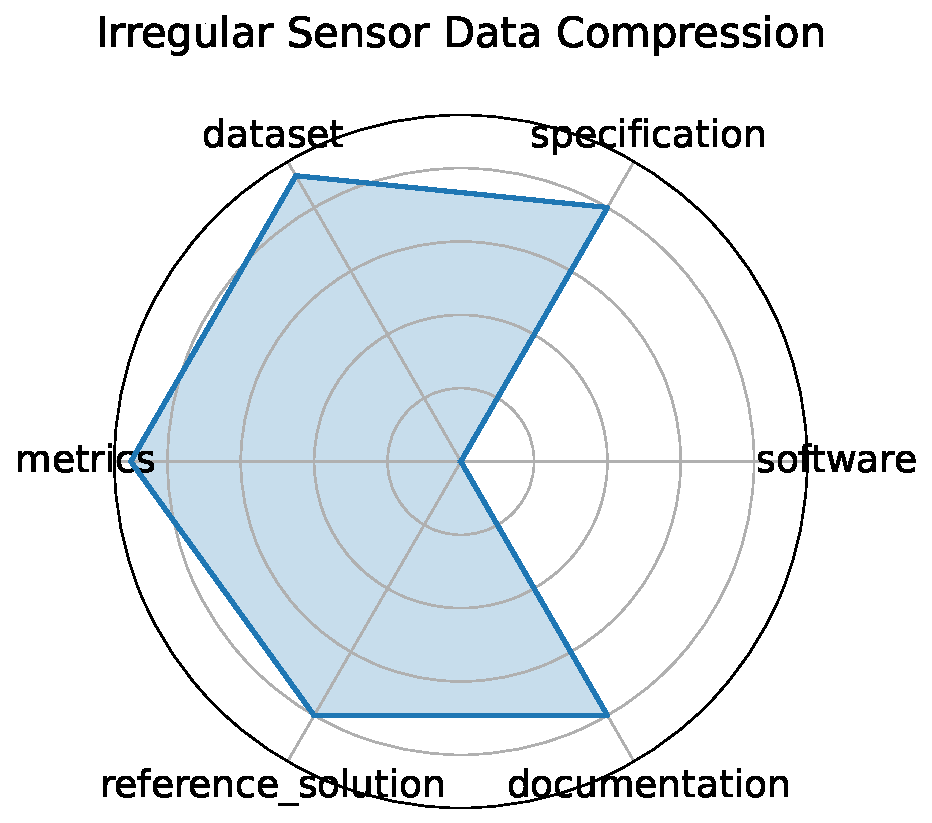
\includegraphics[width=0.2\textwidth]{irregular_sensor_data_compression_radar.pdf}
\end{description}
}}
\clearpage